\documentclass[10pt]{beamer}
\usepackage[utf8]{inputenc}

\usepackage[absolute,overlay]{textpos}
\usepackage{graphicx}
%\usepackage{media9}
\usepackage{booktabs}

\mode<presentation> {
\usetheme{boxes} % When headline is wanted use Dresden theme instead
\usecolortheme{seagull}
\logo{
\includegraphics[height=1.5cm]{ku_logo_dk}}
\setbeamertemplate{footline}[frame number]
% \setbeamertemplate{footline}{
%   \hspace{1em}
%   \hfill
%   \insertframenumber/\inserttotalframenumber
%   \vspace{1em}
%   \hspace{1em}
%   
\includegraphics[height=2cm]{ku_logo_dk}
%   \hspace{1em}
% }
\setbeamertemplate{navigation symbols}{}
\setbeamertemplate{itemize items}[square]
}






%----------------------------------------------------------------------------------------
%	TITLE PAGE
%----------------------------------------------------------------------------------------

\title[Kickstart-kursus] % bottom of every slide
  {Recap Kickstart-kursus i programmering 2022} % title page

\author{\footnotesize{Daniel Spikol} \\
          \footnotesize{\texttt{ds@di.ku.dk}}}

\institute {
DIKU \\ Københavns Universitet
}

\date[August 2022]{20. August 2022}

\begin{document}

\begin{frame}
  \maketitle
\end{frame}

\begin{frame}
   \frametitle{Thanks!}
   	 
\includegraphics[height=8cm]{images/bye22}
\end{frame}

\begin{frame}
\frametitle{Todays Plan}
\begin{itemize}
\item 9.30 - 11.45 Project work
\item 11.45 - 12.30 Lunch
\item 12.30 - 13.00 Final prep
\item 12.30.13.45+ Show and Tell
\item 13.45 - Survey and Thanks!
\end{itemize}
\end{frame}

\begin{frame}
   \frametitle{Show and Tell}
   25 minutes * 3 
   	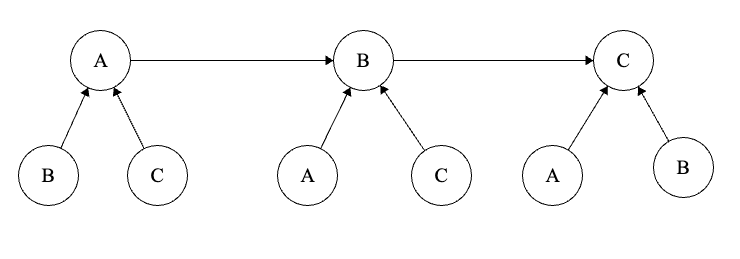
\includegraphics[height=4cm]{images/showtell}
\end{frame}

\begin{frame}
   \frametitle{Remember Grit}
   
\includegraphics[height=7cm]{images/grit}
\end{frame}

\section{Værdier}
\begin{frame}
  \frametitle{De hele tal}

  \begin{itemize}
  \item $\ldots, -3, -2, -1, 0, 1, 2, 3, \ldots$
  \item også kendt som \textit{integers}, \textit{ints} eller \textit{heltal}.
  % \item I matematikken kender vi det som mængden: $\mathbb{Z} = \{ \ldots, -3, -2, -1, 0, 1, 2, 3, \ldots \}$
  \item I Python er der ingen grænser for hvor store tal der kan
    repræsenteres, ulig de fleste andre programmeringssprog.
  \end{itemize}
  
\end{frame}


\begin{frame}
  \frametitle{Operationer på heltal}
  \begin{tabular}{llll}
    \toprule
    \textbf{Operation} & \textbf{Syntaks} & \textbf{Præcedens} & \textbf{Associativitet} \\
    \toprule
    Potensopløftning & \texttt{e1 ** e2} & 1 & Højre \\ \midrule
    Negation & \texttt{- e} & 2 & - \\
    \midrule
    Multiplikation & \texttt{e1 * e2} & 3 & Venstre\\
    Heltals division & \texttt{e1 / e2} & &\\
    Modulus & \texttt{e1 \% e2} & &\\
    \midrule
    Addition & \texttt{e1 + e2} & 4 & Venstre\\
    Subtraktion & \texttt{e1 - e2} & & \\
    \bottomrule
  \end{tabular}

\end{frame}

\begin{frame}
  \frametitle{Floating points (kommatal)}

  \begin{itemize}
  \item $-3.0, -42.3, 0.0, 0.99999996, 13.27$
  \item også kendt som \textit{floating points}, \textit{floats},
    \textit{reals} (reelle tal).
  \item Aldrig helt præcise, så bør bruges med omtanke
  \item Python konverterer automatisk ints til floats, når de bruges i
    en kontekst hvor nødvendigt.
  \end{itemize}
  
\end{frame}

\begin{frame}
  \frametitle{Operationer på floats}
    \begin{tabular}{llll}
    \toprule
    \textbf{Operation} & \textbf{Syntaks} & \textbf{Præcedens} & \textbf{Associativitet} \\
    \toprule
    Potensopløftning & \texttt{e1 ** e2} & 1 & Højre \\ \midrule
    Negation & \texttt{- e} & 2 & - \\
    \midrule
    Multiplikation & \texttt{e1 * e2} & 3 & Venstre\\
    Division & \texttt{e1 / e2} & &\\
    \midrule
    Addition & \texttt{e1 + e2} & 4 & Venstre\\
    Subtraktion & \texttt{e1 - e2} & & \\
    \bottomrule
  \end{tabular}
\end{frame}

\begin{frame}
  \frametitle{Boolske værdier}

  \begin{itemize}
  \item \texttt{True}, \texttt{False}
  \item også kendt som \textit{booleans}, \textit{bools}, eller
    \textit{sandhedsværdier}.
  \end{itemize}

  
\end{frame}

\begin{frame}[fragile]
  \frametitle{Sammenlignings-operationer}

  \begin{tabular}{llll}
    \toprule
    \textbf{Operation} & \textbf{Syntaks} & \textbf{Præcedens} & \textbf{Associativitet} \\
      \toprule
      Større end & \texttt{e1 >= e2} & 5 & Venstre\\
      Mindre end & \texttt{e1 <= e2} & 5 & Venstre\\
      Skarpt større end & \texttt{e1 > e2} & 5 & Venstre\\
      Skarpt mindre end & \texttt{e1 < e2} & 5 & Venstre\\
      Lighed & \texttt{e1 == e2} & 5 & Venstre\\
      Ulighed & \texttt{e1 != e2} & 5 & Venstre\\
    \bottomrule
  \end{tabular}

  \vspace{5mm}
  \textit{OBS! Sammenlign ikke lighed mellem floating points! Check om de er indenfor et interval.}

\begin{verbatim}
>>> 0.1 == 1.0 - 0.9
False
\end{verbatim}
\end{frame}


\begin{frame}
  \frametitle{Operationer på Boolske værdier}

  \begin{tabular}{llll}
    \toprule
    \textbf{Operation} & \textbf{Syntaks} & \textbf{Præcedens} & \textbf{Associativitet} \\
      \toprule
      Logisk ``negation'' & \texttt{not e} & 6 & -\\
      Logisk ``og'' & \texttt{e1 and e2} & 7 & -\\
      Logisk ``eller'' & \texttt{e1 or e2} & 8 & -\\
    \bottomrule
  \end{tabular}
\end{frame}

\begin{frame}
  \frametitle{Strings}

  Værdier:
  \begin{itemize}
  \item \texttt{""}, \texttt{"hello world"}, \texttt{"linje 1\textbackslash nlinje 2"}, \texttt{"\textbackslash""}
  \item \texttt{''}, \texttt{'hello world'}, \texttt{'linje 1\textbackslash nlinje 2'}, \texttt{'"'}
  \end{itemize}
\vspace{5mm}
  \begin{tabular}{llll}
    \toprule
    \textbf{Operation} & \textbf{Syntaks} & \textbf{Præcedens} & \textbf{Associativitet} \\
      \toprule
      Konkatenering & \texttt{e1 + e2} & 4 & -\\
    \bottomrule
  \end{tabular}


\end{frame}

\begin{frame}
  \frametitle{Casting}
  \vspace{5mm}
Cast til int:
\begin{itemize}
\item \texttt{int(50) ==> 50}
\item \texttt{int(7.6) ==> 7}
\item \texttt{int("3") ==> 3}
\end{itemize}

  \vspace{5mm}
Cast til float:
\begin{itemize}
\item \texttt{float(50) ==> 50.0}
\item \texttt{float(7.3) ==> 7.3}
\item \texttt{float("3") ==> 3.0}
\item \texttt{float("4.2") ==> 4.2}
\end{itemize}

\vspace{5mm}
Cast til string:
\begin{itemize}
\item \texttt{str(50) ==> "50"}
\item \texttt{str(7.3) ==> "7.3"}
\item \texttt{str(True) ==> "True"}
\item \texttt{str()} virker også på de fleste andre typer af værdier
\end{itemize}

\end{frame}

\begin{frame}[fragile]
  \frametitle{Betingelser}

Basalt brug:
\begin{verbatim}
  if e:
      ... udføres hvis e evaluerer til True ...
  else:
      ... udføres hvis e evaluerer til False
\end{verbatim}

Udvidet:
\begin{verbatim}
  if e1:
      ... udføres hvis e1 evaluerer til True ...
  elif e2:
      ... udføres hvis e2 evaluerer til True
  else:
      ... hvis hverken e1 eller e2 evaluerer til True ...
\end{verbatim}
\end{frame}

\begin{frame}[fragile]
  \frametitle{Betingelser: Typiske skønhedsfejl}

\begin{verbatim}
  if x == True:
      ...
\end{verbatim}

\vspace{5mm}

\begin{verbatim}
  if x != True:
      ...
\end{verbatim}

\vspace{5mm}

\begin{verbatim}
  if not (x < 100):
      ...
\end{verbatim}

\end{frame}



\begin{frame}[fragile]
  \frametitle{Variabler}

  \begin{itemize}
  \item Variable kan bestå af bogstaver (a-z, A-Z), cifrene (0-9) eller underscore (\_)
  \item Variable må ikke starte med et ciffer
  \item Må ikke navngives med et reserveret ord (fx \texttt{def}, \texttt{if}, \texttt{elif}, \texttt{else}, \texttt{global}, \texttt{True}, \texttt{False}, \texttt{return}, \texttt{and}, \texttt{or}, \texttt{not}, ...)
  \item Variabler er \textit{case sensitive} (variablen \texttt{ABc} er forskellig fra \texttt{ABC})
  \item Variabler defineres første gang de sættes
  \end{itemize}

  \vspace{5mm}
Eksempler:
\begin{verbatim}
foo = 17 + 42 / 6
bar = foo * 2.0
baz = bar < 10
\end{verbatim}

\end{frame}

\begin{frame}[fragile,fragile,fragile]
  \frametitle{Funktioner}
  \begin{itemize}
  \item Funktioner følger samme navngivningsregler som variabler
  \item Du kan ikke have en variabel og en funktion der hedder det
    samme, da vil den senest definerede overskrive (de er i samme ``navnerum'')
  \end{itemize}

Eksempel:
\begin{verbatim}
def kvadrat(x):
    return x * x

def kvadratsum(a, b):
    return kvadrat(a) + kvadrat(b)

kvadratsum(1+2, 4)
\end{verbatim}

\end{frame}


\begin{frame}[fragile]
  \frametitle{Globale vs. lokale variabler}
Eksempel 1:
\begin{verbatim}
  foo = 42
  def minfunktion():
      global foo
      foo = 20
  minfunktion()
  # variablen "foo" er nu sat til 20
\end{verbatim}

~

\noindent
Eksempel 2:
\begin{verbatim}
  foo = 42
  def minfunktion():
      foo = 20
  minfunktion()
  # variablen "foo" er stadig 42
\end{verbatim}
Her er der to variabler med samme navn \texttt{foo}.

\end{frame}



\begin{frame}[fragile,fragile]
  \frametitle{Scoping, virkefelter}
  \framesubtitle{Hvilke variabler og funktioner er synlige hvor?}

  \begin{align*}
    &\texttt{variabel1 = ...} \\
    &\fbox{A} \\
    &\texttt{def~}\texttt{funktion1(argument0, argument1)}: \\
    &\texttt{~~~~}\texttt{variabel2 = ...} \\
    &\texttt{~~~~}\fbox{B} \\
    &\fbox{C}
  \end{align*}

  \begin{itemize}
  \item \texttt{variabel1} er synlig i \fbox{A}, \fbox{B}, \fbox{C}
  \item \texttt{argument0} og \texttt{argument1} er synlige i \fbox{B}
  \item \texttt{variabel2} er synlig i \fbox{B}
  \item \texttt{funktion1} er synlig i \fbox{B}, \fbox{C}
  \end{itemize}
  
\end{frame}

\end{document}